\section{PSoC Master} \label{sec:PSoC_Master_design}

På Figur \ref{fig:Master_PSoC_klassediagram} ses klassediagrammet for Master PSoC. Der er blevet designet 4 klasser der håndterer hver sin del af arbejdet, som masteren skal udføre. Der er valgt to boundaryklasser, som håndterer kommunikation over hhv. UART og \IIC. Udover dette er der en domæneklasse, som indeholder alle de målte dataværdier, der er modtaget af sensorerne. 

\begin{figure}[h]
\centering 
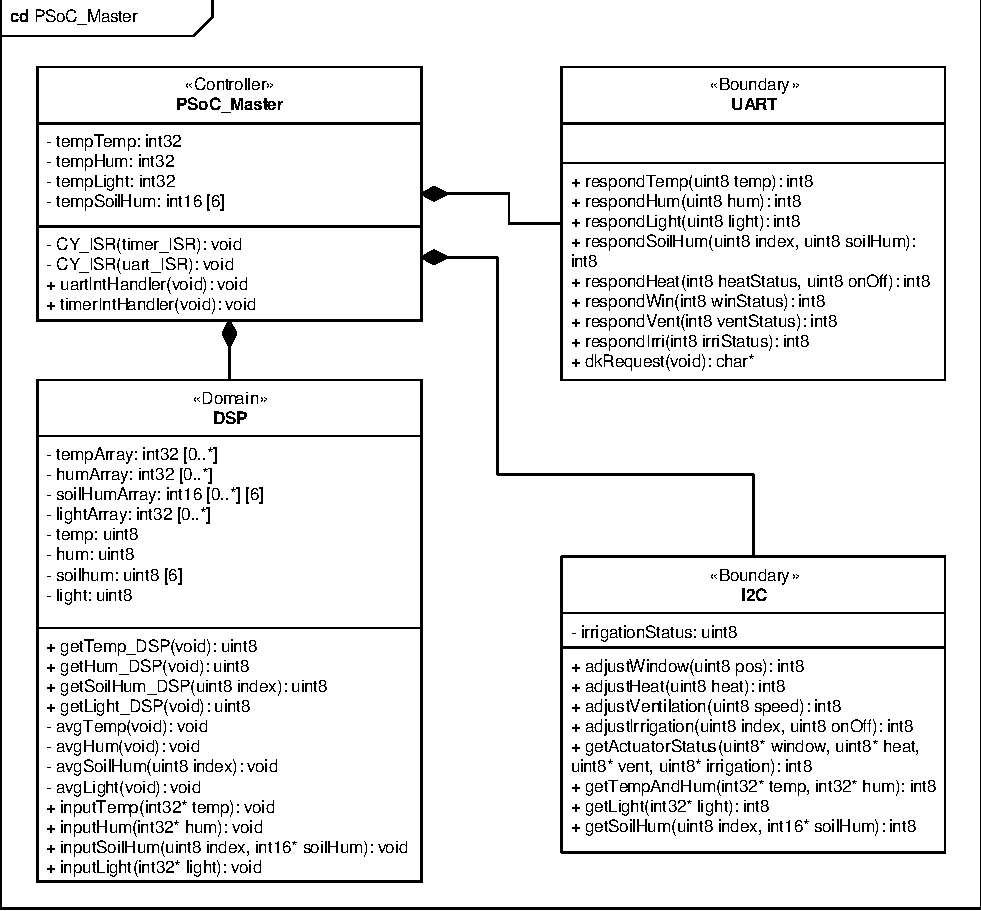
\includegraphics[width={\textwidth}, trim=0 0 0 0, clip=true] {../fig/cd_PSoC_master.pdf}
\caption{Klassediagram for Master PSoC}
\label{fig:Master_PSoC_klassediagram}
\end{figure}

\clearpage

\subsection{Klassebeskrivelser}

%++++++++++++ Controller PSoC Master klassen ++++++++++++++
\subsubsection{Controllerklasse PSoC\_Master}

\textbf{Attributter}

\begin{table}[h]
\begin{tabularx}{\textwidth}{| >{\raggedright\arraybackslash}X | >{\raggedright\arraybackslash}X | >{\raggedright\arraybackslash}p{10 cm} |} \hline
Navn & Type & Beskrivelse \\\hline
\texttt{tempTemp} & \texttt{int32} & Midlertidig variabel til opbevaring af temperatur. \\\hline
\texttt{tempHum} & \texttt{int32} & Midlertidig variabel til opbevaring af luftfugtighed. \\\hline
\texttt{tempLight} & \texttt{int32} & Midlertidig variabel til opbevaring af lysintensitet. \\\hline
\texttt{tempSoilHum} & \texttt{int16 [6]} & Array af midlertidige variabler til opbevaring af jordfugtighed. \\\hline
\end{tabularx}
\caption{Attributter for klassen PSoC\_Master}
\label{table:PSoC_Master_attributter}
\end{table}

\textbf{Metoder}

%========================= CY_ISR(timer_ISR) ==============

\begin{table}[h]
\begin{tabularx}{\textwidth}{| >{\raggedright\arraybackslash}p{2.5 cm} | >{\raggedright\arraybackslash}X |} \hline
Prototype & \texttt{void CY\_ISR(timer\_ISR)} \\\hline
Parametre & \texttt{timer\_ISR} \newline Vector for den givne interrupt servicerutine. \\\hline
Returværdi & - \\\hline
Beskrivelse & Denne interrupt service rutine bliver kaldt, når en ønsket tidsperiode er forløbet. Rutinen kalder metoder i boundaryklassen \IIC, der varetager indhentning af data fra sensorer.  \\\hline
\end{tabularx}
\caption{CY\_ISR(timer\_ISR)}
\label{table:CY_ISR(timer_ISR)}
\end{table}

%========================= CY_ISR(uart_ISR) ==============

\begin{table}[h]
\begin{tabularx}{\textwidth}{| >{\raggedright\arraybackslash}p{2.5 cm} | >{\raggedright\arraybackslash}X |} \hline
Prototype & \texttt{void CY\_ISR(uart\_ISR)} \\\hline
Parametre & \texttt{uart\_ISR} \newline 
Vector for den givne interrupt servicerutine. \\\hline
Returværdi & - \\\hline
Beskrivelse & Denne interrupt service rutine bliver kaldt, når der modtages noget på UART fra DevKit8000. Rutinen kalder metoder i boundaryklasserne \IIC og UART. Formålet med interrupten er at håndtere forskellige typer af forespørgsler. \\\hline
\end{tabularx}
\caption{CY\_ISR(uart\_ISR)}
\label{table:CY_ISR(uart_ISR)}
\end{table}

%========================= timerIntHandler ==============

\begin{table}[h]
\begin{tabularx}{\textwidth}{| >{\raggedright\arraybackslash}p{2.5 cm} | >{\raggedright\arraybackslash}X |} \hline
Prototype & \texttt{void timerIntHandler(void)} \\\hline
Parametre & - \\\hline
Returværdi & - \\\hline
Beskrivelse & Kontrollerer et flag sat af timer\_ISR. Hvis flag er sat, spørger den på \IIC om sensor-værdier. \\\hline
\end{tabularx}
\caption{timerIntHandler()}
\label{table:timerIntHandler()}
\end{table}

%========================= uartIntHandler ==============

\begin{table}[h]
\begin{tabularx}{\textwidth}{| >{\raggedright\arraybackslash}p{2.5 cm} | >{\raggedright\arraybackslash}X |} \hline
Prototype & \texttt{void uartIntHandler(void)} \\\hline
Parametre & - \\\hline
Returværdi & - \\\hline
Beskrivelse & Kontrollerer et flag sat af uart\_ISR. Hvis flaget er sat, spørger den på \IIC om sensor-værdier. \\\hline
\end{tabularx}
\caption{timerIntHandler()}
\label{table:timerIntHandler()}
\end{table}

%========================= FLERE UART FUNKTIONER ==============

\newpage

\subsubsection{Boundaryklasse UART}
%+++++++++++++++++++++++++ Boundary UART ++++++++++++++++++++
\textbf{Metoder}

%========================= respondTemp ==============

\begin{table}[h]
\begin{tabularx}{\textwidth}{| >{\raggedright\arraybackslash}p{2.5 cm} | >{\raggedright\arraybackslash}X |} \hline
Prototype & \texttt{int8 respondTemp(uint8 temp)} \\\hline
Parametre & \texttt{uint8 temp} \newline
Den nyeste midlede temperatur hentet fra domæneklassen DSP. 
 \\\hline
Returværdi & \texttt{int8} \newline
Er denne værdi nul er der blevet returneret en gyldig værdi. Hvis værdien er -1 er der blevet returneret ’XT’ over UART. \\\hline
Beskrivelse & Hvis parameter værdien ligger inden for decimalværdien 1-200 (begge inklusive), skal metoden sende en char ’T’, efterfulgt af temp parameteren, over UART. Er værdien er lig nul, skal metoden sende strengen ”XT".   \\\hline
\end{tabularx}
\caption{respondTemp}
\label{table:respondTemp}
\end{table}

%========================= respondHum ==============

\begin{table}[h]
\begin{tabularx}{\textwidth}{| >{\raggedright\arraybackslash}p{2.5 cm} | >{\raggedright\arraybackslash}X |} \hline
Prototype & \texttt{ int8 respondHum(uint8 hum)} \\\hline
Parametre & \texttt{uint8 hum} \newline
Den nyeste midlede luftfugtighed hentet fra domæneklassen DSP. 
 \\\hline
Returværdi & \texttt{int8} \newline
Er denne værdi nul er der blevet returneret en gyldig værdi. Hvis værdien er -1 er der blevet returneret ’XA’ over UART. \\\hline
Beskrivelse & Hvis parameter værdien ligger inden for decimalværdien 1-100 (begge inklusive), skal metoden sende en char ’A’, efterfulgt af hum parameteren, over UART. Hvis værdien er lig nul, skal metoden sende strengen ”XA".    \\\hline
\end{tabularx}
\caption{respondHum}
\label{table:respondHum}
\end{table}

%========================= respondLight ==============

\begin{table}[h]
\begin{tabularx}{\textwidth}{| >{\raggedright\arraybackslash}p{2.5 cm} | >{\raggedright\arraybackslash}X |} \hline
Prototype & \texttt{int8 respondLight(uint8 light)} \\\hline
Parametre & \texttt{uint8 light} \newline
Den nyeste midlede lysintensitet hentet fra domæneklassen DSP. 
 \\\hline
Returværdi & \texttt{int8} \newline
Er denne værdi nul er der blevet returneret en gyldig værdi. Hvis værdien er -1 er der blevet returneret ’XL’ over UART.\\\hline
Beskrivelse & Hvis parameter værdien ligger inden for decimalværdien 1-100 (begge inklusive), skal metoden sende en char ’L’ efterfulgt af light parameteren over UART. Hvis værdien er lig nul, skal metoden sende strengen ”XL".     \\\hline
\end{tabularx}
\caption{respondLight}
\label{table:respondLight}
\end{table}

%========================= respondSoilHum ==============

\begin{table}[h]
\begin{tabularx}{\textwidth}{| >{\raggedright\arraybackslash}p{2.5 cm} | >{\raggedright\arraybackslash}X |} \hline
Prototype & \texttt{int8 respondSoilHum(uint8 index, uint8 soilHum)} \\\hline
Parametre & \texttt{uint8 soilHum} \newline
Den nyeste midlede jordfugtighed hentet fra domæneklassen DSP. \newline
\texttt{uint8 index} \newline
Indexet fortæller hvilket sensornummer der svares fra. Kan være værdierne 0-5. \\\hline
Returværdi & \texttt{int8} \newline
Er denne værdi nul er der blevet returneret en gyldig værdi. Hvis værdien er -1 er der blevet returneret ’XS’ over UART.\\\hline
Beskrivelse & Hvis parameter værdien ligger inden for decimalværdien 1-10 (begge inklusive), skal metoden sende en char ’S’, efterfulgt af index og soilHum parametrene over UART. Hvis værdien for soilHum er lig nul, skal metoden sende strengen ”XS". \\\hline
\end{tabularx}
\caption{respondSoilHum}
\label{table:respondSoilHum}
\end{table}

%========================= respondHeat ==============

\begin{table}[h]
\begin{tabularx}{\textwidth}{| >{\raggedright\arraybackslash}p{2.5 cm} | >{\raggedright\arraybackslash}X |} \hline
Prototype & \texttt{int8 respondHeat(uint8 heatStatus, uint8 On)} \\\hline
Parametre & \texttt{uint8 heatStatus} \newline
Returværdien fra funktionen adjustHeat i boundaryklassen \IIC; fortæller om kommunikationen over \IIC er gået godt. \newline
\texttt{uint8 On} \newline
Returværdi til UART afhængig af hvilken kommando, der blev kaldt. 0 = off, 0 != on.
 \\\hline
Returværdi & \texttt{int8} \newline
Er denne værdi nul er kommunikationen over \IIC gennemført. Hvis værdien er
-1 er der blevet returneret en værdi tilsvarene requesten fra DevKit8000 over UART (se UART protokol side \pageref{UART_Protokol}) og der er sket en fejl i kommunikationen over \IIC.
\\\hline
Beskrivelse & Hvis parameter værdien er lig nul, sendes en char tilsvarene requesten over UART. Hvis værdien er lig -1, sendes sendes en tilsvarene fejlmeddelelse. \\\hline
\end{tabularx}
\caption{respondHeat}
\label{table:respondHeat}
\end{table}

%========================= respondWin ==============

\begin{table}[h]
\begin{tabularx}{\textwidth}{| >{\raggedright\arraybackslash}p{2.5 cm} | >{\raggedright\arraybackslash}X |} \hline
Prototype & \texttt{int8 respondWin(int8 winStatus)} \\\hline
Parametre & \texttt{int8 winStatus} \newline
Returværdien fra funktionen adjustWin i boundaryklassen \IIC. Fortæller om kommunikationen via. \IIC til vinduesaktuatoren er forløbet godt.  
 \\\hline
Returværdi & \texttt{int8} \newline
Er denne værdi nul er kommunikationen over \IIC gennemført. Hvis værdien er -1 er der blevet returneret ’XK’ over UART og der er sket en fejl i kommunikationen over \IIC.\\\hline
Beskrivelse & Hvis parameter værdien er lig nul, sendes en char ’K’ over UART. Hvis værdien er lig -1, sendes strengen ”XK". \\\hline
\end{tabularx}
\caption{respondWin}
\label{table:respondWin}
\end{table}

%========================= respondVent ==============

\begin{table}[h]
\begin{tabularx}{\textwidth}{| >{\raggedright\arraybackslash}p{2.5 cm} | >{\raggedright\arraybackslash}X |} \hline
Prototype & \texttt{int8 respondVent(int8 ventStatus)} \\\hline
Parametre & \texttt{int8 ventStatus} \newline
Returværdien fra funktionen adjustVent i boundaryklassen \IIC. Fortæller om kommunikationen via \IIC til ventilatoraktuatoren er forløbet uden problemer.   
 \\\hline
Returværdi & \texttt{int8} \newline
Er denne værdi 0, er kommunikationen over \IIC gennemført. Hvis værdien er 
-1 er der blevet returneret ’XV’ over UART og der er sket en fejl i kommunikationen over \IIC.
\\\hline
Beskrivelse & Hvis parameterværdien er lig nul, sendes en char ’V’ over UART, hvilket indikerer at det er gået godt. Hvis værdien er lig -1, sendes strengen ”XV". \\\hline
\end{tabularx}
\caption{respondVent}
\label{table:respondVent}
\end{table}

%========================= respondIrri ==============

\begin{table}[h]
\begin{tabularx}{\textwidth}{| >{\raggedright\arraybackslash}p{2.5 cm} | >{\raggedright\arraybackslash}X |} \hline
Prototype & \texttt{int8 respondIrri(int8 irriStatus)} \\\hline
Parametre & \texttt{int8 irriStatus} \newline
Returværdien fra funktionen adjustIrrigation i boundaryklassen \IIC. Fortæller om kommunikationen via \IIC til irrigationsaktuatoren er forløbet uden problemer.   
 \\\hline
Returværdi & \texttt{int8} \newline
Er denne værdi nul, er kommunikationen over \IIC gennemført. Hvis værdien er 
-1 er der blevet returneret ’XF’ over UART og der er sket en fejl i kommunikationen over \IIC.
\\\hline
Beskrivelse & Hvis parameterværdien er lig nul, sendes en char ’F’ over UART, hvilket indikerer at det er gået godt. Hvis værdien er lig 
-1, sendes strengen ”XF". \\\hline
\end{tabularx}
\caption{respondIrri}
\label{table:respondIrri}
\end{table}

\clearpage

%+++++++++++++++++++++++++ I2C klassen ++++++++++++++
\subsubsection{Boundaryklasse \IIC}

\textbf{Attributter}

\begin{table}[h]
\begin{tabularx}{\textwidth}{| >{\raggedright\arraybackslash}X | >{\raggedright\arraybackslash}X | >{\raggedright\arraybackslash}p{8 cm} |} \hline
Navn & Type & Beskrivelse \\\hline
\texttt{irrigationStatus} & \texttt{uint8} & Indeholder den aktuelle status for vandingsaktuatorer (tændt eller slukkede). Bit 0 – 5 er hhv. aktuatorerne fra 1 – 6. Nul betyder slukket og et betyder tændt. \\\hline
\end{tabularx}
\caption{Attributter for klassen \IIC}
\label{table:IIC_attributter}
\end{table}

\textbf{Metoder}

%========================= adjustWindow ==============

\begin{table}[h]
\begin{tabularx}{\textwidth}{| >{\raggedright\arraybackslash}p{2.5 cm} | >{\raggedright\arraybackslash}X |} \hline
Prototype & \texttt{int8 adjustWindow(uint8 pos)} \\\hline
Parametre & \texttt{uint8 pos} \newline 
Den ønskede status for vinduet. Kan være hhv. 0xFF for åben og 0x00 for lukket. \\\hline
Returværdi & \texttt{int8} \newline
Er værdien 0, er kommunikation via \IIC gået godt. Hvis værdien er -1, er der sket en fejl. \\\hline
Beskrivelse & Metoden kan justere positionen for vinduet i drivhuset. Sender kommandoen ”WriteAdjustWindow” via \IIC bussen (se \IIC protokol på side \pageref{sec:I2C_protokol}). \\\hline
\end{tabularx}
\caption{adjustWindow}
\label{table:adjustWindow}
\end{table}

%========================= adjustHeat ==============

\begin{table}[h]
\begin{tabularx}{\textwidth}{| >{\raggedright\arraybackslash}p{2.5 cm} | >{\raggedright\arraybackslash}X |} \hline
Prototype & \texttt{int8 adjustHeat(uint8 heat)} \\\hline
Parametre & \texttt{uint8 heat} \newline 
Bestemmer intensiteten af varmen, 0x00 er ingen varme, 0xFF er fuld varme. \\\hline
Returværdi & \texttt{int8} \newline
Er værdien 0, er kommunikation via \IIC gået godt. Hvis værdien er -1, er der sket en fejl (se \IIC protokol på side \pageref{sec:I2C_protokol}). \\\hline
Beskrivelse & Slukker eller tænder for varmeaktuatoren. Sender kommandoen ”WriteAdjustHeat” via \IIC bussen (se \IIC protokol på side \pageref{sec:I2C_protokol}). \\\hline
\end{tabularx}
\caption{adjustHeat}
\label{table:adjustHeat}
\end{table}

%========================= adjustVentilation ==============

\begin{table}[h]
\begin{tabularx}{\textwidth}{| >{\raggedright\arraybackslash}p{2.5 cm} | >{\raggedright\arraybackslash}X |} \hline
Prototype & \texttt{int8 adjustVentilation(uint8 speed)} \\\hline
Parametre & \texttt{uint8 speed} \newline 
Beskriver ventilatoraktuatornes tilstand. 0x00 svarer til slukket og 0xFF svarer til fuld hastighed. \\\hline
Returværdi & \texttt{int8} \newline
Er værdien 0, er kommunikation via \IIC gået godt. Hvis værdien er -1, er der sket en fejl (se \IIC protokol på side \pageref{sec:I2C_protokol}). \\\hline
Beskrivelse & Slukker eller tænder for ventilation. Sender kommandoen ”WriteAdjustVentilation” via \IIC bussen (se \IIC protokol på side \pageref{sec:I2C_protokol}). \\\hline
\end{tabularx}
\caption{adjustVentilation}
\label{table:adjustVent}
\end{table}

%========================= adjustIrrigation ==============

\begin{table}[h]
\begin{tabularx}{\textwidth}{| >{\raggedright\arraybackslash}p{2.5 cm} | >{\raggedright\arraybackslash}X |} \hline
Prototype & \texttt{int8 adjustIrrigation(uint8 index, uint8 on)} \\\hline
Parametre & \texttt{uint8 index} \newline 
Indeksoperator for hvilken vandingsaktuator der skal aktiveres. Første = 0, sidste = 5. \newline
\texttt{uint8 on} \newline
Beskriver tilstanden for vandingsaktuatoren. 0x00 svarer til slukket og 0xFF svarer til tændt. \\\hline
Returværdi & \texttt{int8} \newline
Er værdien 0, er kommunikation via \IIC gået godt. Hvis værdien er -1, er der sket en fejl (se \IIC protokol på side \pageref{sec:I2C_protokol}). \\\hline
Beskrivelse & Slukker eller tænder for individuelle vandingsaktuatorer. Sender kommandoen ”WriteAdjustIrrigation” via \IIC bussen (se \IIC protokol på side \pageref{sec:I2C_protokol}). \\\hline
\end{tabularx}
\caption{adjustIrrigation}
\label{table:adjustIrri}
\end{table}

%========================= getActuatorStatus ==============

\begin{table}[h]
\begin{tabularx}{\textwidth}{| >{\raggedright\arraybackslash}p{2.5 cm} | >{\raggedright\arraybackslash}X |} \hline
Prototype & \texttt{int8 getActuatorStatus(uint8* window, uint8* heat, \newline uint8* vent, uint8* irrigation)} \\\hline
Parametre & \texttt{uint8* window} \newline 
Pointer til variable som status for vinduet skrives i. \newline
\texttt{uint8* heat} \newline
Pointer til variable som status for varmelegeme skrives i. \newline
\texttt{uint8 uint8* vent} \newline
Pointer til variable som status for ventilator skrives i. \newline
\texttt{uint8* irrigation} \newline
Pointer til variable som status for vandingsaktuatorer skrives i. \\\hline
Returværdi & \texttt{int8} \newline
Er værdien 0, er kommunikation via \IIC gået godt. Hvis værdien er -1, er der sket en fejl. \\\hline
Beskrivelse & Giver overblik over aktuatorslavens tilstand. Der henvises til \IIC protokollen på side \pageref{sec:I2C_protokol} for yderligere information. \\\hline
\end{tabularx}
\caption{getActuatorStatus}
\label{table:getActuatorStatus}
\end{table}

%========================= getTempAndHum ==============

\begin{table}[h]
\begin{tabularx}{\textwidth}{| >{\raggedright\arraybackslash}p{2.5 cm} | >{\raggedright\arraybackslash}X |} \hline
Prototype & \texttt{int8 getTempAndHum(int32* temp, int32* hum)} \\\hline
Parametre & \texttt{int32* temp} \newline 
Pointer til variabel, hvori ubehandlet temperaturdata i drivhuset skrives. \newline
\texttt{int32* hum} \newline
Pointer til variabel, hvori ubehandlet luftfugtighedsdata i drivhuset skrives. \newline \newline
Omregningsformel kan findes i databladet for sensoren. \cite{lib:TempHum_I2C} \\\hline
Returværdi & \texttt{int8} \newline
Er værdien 0, er kommunikation via \IIC gået godt. Hvis værdien er -1, er der sket en fejl. \\\hline
Beskrivelse & Metoden skriver ubehandlet data fra sensoren i to variable. Der henvises til \IIC protokollen på side \pageref{sec:I2C_protokol} og til sensorens datablad \cite{lib:TempHum_I2C} for yderligere information. \\\hline
\end{tabularx}
\caption{getTempAndHum}
\label{table:getTempAndHum}
\end{table}

%========================= getLight ==============

\begin{table}[h]
\begin{tabularx}{\textwidth}{| >{\raggedright\arraybackslash}p{2.5 cm} | >{\raggedright\arraybackslash}X |} \hline
Prototype & \texttt{int8 getLight(int32* light)} \\\hline
Parametre & \texttt{int32* light} \newline 
Pointer til variabel, hvori ubehandlet lysintensitetsdata i drivhuset skrives. \newline \newline
Omregningsformel kan findes i databladet for sensoren. \cite{lib:LightSens}. \\\hline
Returværdi & \texttt{int8} \newline
Er værdien 0, er kommunikation via \IIC gået godt. Hvis værdien er -1, er der sket en fejl. \\\hline
Beskrivelse & Metoden skriver ubehandlet data fra sensoren i en variabel. Der henvises til \IIC protokollen på side \pageref{sec:I2C_protokol} og til sensorens datablad \cite{lib:LightSens} for yderligere information. \\\hline
\end{tabularx}
\caption{getLight}
\label{table:getLight}
\end{table}

%========================= getSoilHum ==============

\begin{table}[h]
\begin{tabularx}{\textwidth}{| >{\raggedright\arraybackslash}p{2.5 cm} | >{\raggedright\arraybackslash}X |} \hline
Prototype & \texttt{int8 getSoilHum(uint8 index, int16* soilHum)} \\\hline
Parametre & \texttt{uint8* index} \newline 
Indeks for hvilken jordfugtsensor der ønskes at læse fra, den første sensor hedder 0 og den sidste 5. \newline
\texttt{int16* soilHum} \newline 
Pointer til variabel, hvori ubehandlet jordfugtighedsdata i drivhuset skrives. \\\hline
Returværdi & \texttt{int8} \newline
Er værdien 0, er kommunikation via \IIC gået godt. Hvis værdien er -1, er der sket en fejl. \\\hline
Beskrivelse & Metoden skriver ubehandlet data fra sensoren i en variabel. \\\hline
%Der henvises til \IIC protokollen på side \pageref{sec:I2C_protokol} for yderligere information.
%TODO Find ud af noget dokumentation omkring soilHumsensoren og referer til det her?!
\end{tabularx}
\caption{getSoilHum}
\label{table:getSoilHum_IIC}
\end{table}

\clearpage

%+++++++++++++++++++++++++ DSP klassen ++++++++++++++
\subsubsection{Domainklasse DSP}

\textbf{Attributter}

\begin{table}[h]
\begin{tabularx}{\textwidth}{| >{\raggedright\arraybackslash}X | >{\raggedright\arraybackslash}X | >{\raggedright\arraybackslash}p{8 cm} |} \hline
Navn & Type & Beskrivelse \\\hline
\texttt{tempArray} & \texttt{int32} & Array der indeholder måleværdier fra temperaturmåler. \\\hline
\texttt{humArray} & \texttt{int32} & Array der indeholder måleværdier fra fugtighedsmåler. \\\hline
\texttt{soilHumArray} & \texttt{int16} & To-dimentionelt array der indeholder målinger fra jordfugtsensorerne. \\\hline
\texttt{lightArray} & \texttt{int32} & Array der indeholder måleværdier fra lyssensoren. \\\hline
\texttt{temp} & \texttt{uint8} & Variabel der indeholder den midlede og konverterede værdi af temperaturen, som DevKit8000 kan efterspørge. \\\hline
\texttt{hum} & \texttt{uint8} & Variabel der indeholder den midlede værdi af fugtigheden, som DevKit8000 kan efterspørge. \\\hline
\texttt{soilHum} & \texttt{uint8} & Variabel der indeholder den midlede værdi af jordfugtigheden, som DevKit8000 kan efterspørge. \\\hline
\texttt{light} & \texttt{uint8} & Variabel der indeholder den midlede værdi af lysintensiteten, som DevKit8000 kan efterspørge. \\\hline
\end{tabularx}
\caption{Attributter for klassen DSP}
\label{table:DSP_attributter}
\end{table}

\begin{table}[h]
\begin{tabularx}{\textwidth}{| >{\raggedright\arraybackslash}p{2.5 cm} |  >{\raggedright\arraybackslash}p{2.9 cm} | >{\raggedright\arraybackslash}X |} \hline
Navn & Type & Beskrivelse \\\hline
\texttt{tempArray} & \texttt{int32[0..*]} & Pointer til et array på en given størrelse, som indeholder ubearbejdede målinger af temperaturen, indhentet fra boundaryklassen \IIC. \\\hline
\texttt{humArray} & \texttt{int32[0..*]} & Pointer til et array på en given størrelse, som indeholder ubearbejdede målinger af luftfugtigheden, indhentet fra boundaryklassen \IIC. \\\hline
\texttt{soilHumArray} & \texttt{int16[0..*][6]} & Todimensionelt array på 6 pladser, som indeholder arrays med ubearbejdede målinger af jordfugtigheden, indhentet fra boundaryklassen \IIC. \\\hline
\texttt{lightArray} & \texttt{int32[0..*]} & Pointer til et array på en given størrelse, som indeholder ubearbejdede målinger af luftfugtigheden, indhentet fra boundaryklassen \IIC. \\\hline
\texttt{temp} & \texttt{uint8} & Indeholder den nyeste midlede temperaturværdi. \\\hline
\texttt{hum} & \texttt{uint8} & Indeholder den nyeste midlede luftfugtighedsværdi. \\\hline
\texttt{soilHum} & \texttt{uint8[6]} & Array der indeholder de nyeste midlede jordfugtighedsværdier. \\\hline
\texttt{light} & \texttt{uint8} & Indeholder den nyeste midlede lysintensitetsværdi. \\\hline
\end{tabularx}
\caption{Attributter for klassen \IIC}
\label{table:DSP_attributter}
\end{table}

\textbf{Metoder}

%========================= getTemp ==============

\begin{table}[h]
\begin{tabularx}{\textwidth}{| >{\raggedright\arraybackslash}p{2.5 cm} | >{\raggedright\arraybackslash}X |} \hline
Prototype & \texttt{int8 getTemp\_DSP(void)} \\\hline
Parametre & - \\\hline
Returværdi & \texttt{int8} \newline
Metoden returnerer variablen temp. \\\hline
Beskrivelse & Kan bruges til at hente den midlede temperatur, der skal sendes via UART til DevKit8000. \\\hline
\end{tabularx}
\caption{getTemp\_DSP}
\label{table:getTemp_DSP}
\end{table}

%========================= getHum ==============

\begin{table}[h]
\begin{tabularx}{\textwidth}{| >{\raggedright\arraybackslash}p{2.5 cm} | >{\raggedright\arraybackslash}X |} \hline
Prototype & \texttt{int8 getHum\_DSP(void)} \\\hline
Parametre & - \\\hline
Returværdi & \texttt{int8} \newline
Metoden returnerer variablen hum. \\\hline
Beskrivelse & Kan bruges til at hente den midlede luftfugtighed, der skal sendes via UART til DevKit8000. \\\hline
\end{tabularx}
\caption{getHum\_DSP}
\label{table:getHum_DSP}
\end{table}

%========================= getSoilHum ==============

\clearpage

\begin{table}[h]
\begin{tabularx}{\textwidth}{| >{\raggedright\arraybackslash}p{2.5 cm} | >{\raggedright\arraybackslash}X |} \hline
Prototype & \texttt{int8 getSoilHum\_DSP(uint8 index)} \\\hline
Parametre & \texttt{uint8 index} \newline
Fortæller hvilken jordfugtighedssensor der returneres værdier fra. \\\hline
Returværdi & \texttt{int8} \newline
Returnerer variablen soilHum der tilsvarer parametret index. \\\hline
Beskrivelse & Metoden bruges til at hente den midlede jordfugtighed, der skal sendes via UART til DevKit8000. \\\hline
\end{tabularx}
\caption{getSoilHum\_DSP}
\label{table:getSoilHum_DSP}
\end{table}

%========================= getLight ==============

\begin{table}[h]
\begin{tabularx}{\textwidth}{| >{\raggedright\arraybackslash}p{2.5 cm} | >{\raggedright\arraybackslash}X |} \hline
Prototype & \texttt{int8 getLight\_DSP(void)} \\\hline
Parametre & - \\\hline
Returværdi & \texttt{int8} \newline
Metoden returnerer variablen light. \\\hline
Beskrivelse & Kan bruges til at hente den midlede lysintensitet, der skal sendes via UART til DevKit8000. \\\hline
\end{tabularx}
\caption{getLight\_DSP}
\label{table:getLight_DSP}
\end{table}

%========================= avgTemp ==============

\begin{table}[h]
\begin{tabularx}{\textwidth}{| >{\raggedright\arraybackslash}p{2.5 cm} | >{\raggedright\arraybackslash}X |} \hline
Prototype & \texttt{void avgTemp(void)} \\\hline
Parametre & - \\\hline
Returværdi & - \\\hline
Beskrivelse & Metoden beregner en middelværdi for temperaturene i tempArray og konverterer svaret til et passende format og gemmer det i \texttt{temp}. Se UART protokollen side \pageref{UART_Protokol} og databladet for temperatursensoren \cite{lib:TempHum_I2C}.  \\ \hline
\end{tabularx}
\caption{avgTemp}
\label{table:avgTemp}
\end{table}

%========================= avgHum ==============

\begin{table}[h]
\begin{tabularx}{\textwidth}{| >{\raggedright\arraybackslash}p{2.5 cm} | >{\raggedright\arraybackslash}X |} \hline
Prototype & \texttt{void avgHum(void)} \\\hline
Parametre & - \\\hline
Returværdi & - \\\hline
Beskrivelse & Metoden beregner en middelværdi for luftfugtigheden i humArray og konverterer svaret til et passende format og gemmer det i \texttt{hum}. Se UART protokollen side \pageref{UART_Protokol} og databladet for temperatursensoren \cite{lib:TempHum_I2C}.  \\ \hline
\end{tabularx}
\caption{avgHum}
\label{table:avgHum}
\end{table}

%========================= avgSoilHum ==============

\begin{table}[h]
\begin{tabularx}{\textwidth}{| >{\raggedright\arraybackslash}p{2.5 cm} | >{\raggedright\arraybackslash}X |} \hline
Prototype & \texttt{void avgSoilHum(void)} \\\hline
Parametre & - \\\hline
Returværdi & - \\\hline
Beskrivelse & Metoden beregner en middelværdi for hver sæt værdier for jordfugtighed i soilHumArray og konverterer svaret til et passende format og gemmer det i \texttt{soilHum} arrayet. Se UART protokollen side \pageref{UART_Protokol}.  \\ \hline
\end{tabularx}
\caption{avgSoilHum}
\label{table:avgSoilHum}
\end{table}

%========================= avgLight ==============

\begin{table}[h]
\begin{tabularx}{\textwidth}{| >{\raggedright\arraybackslash}p{2.5 cm} | >{\raggedright\arraybackslash}X |} \hline
Prototype & \texttt{void avgLight(void)} \\\hline
Parametre & - \\\hline
Returværdi & - \\\hline
Beskrivelse & Metoden beregner en middelværdi for lysintensiten i lightArray og konverterer svaret til et passende format og gemmer det i \texttt{light}. Se UART protokollen side \pageref{UART_Protokol} og databladet for temperatursensoren \cite{lib:LightSens}.  \\ \hline
\end{tabularx}
\caption{avgLight}
\label{table:avgLight}
\end{table}

%========================= inputTemp ==============

\begin{table}[h]
\begin{tabularx}{\textwidth}{| >{\raggedright\arraybackslash}p{2.5 cm} | >{\raggedright\arraybackslash}X |} \hline
Prototype & \texttt{void inputTemp(int32* temp)} \\\hline
Parametre & \texttt{int32* temp} \newline
En pointer til en variabel der ønskes indlæst i tempArray. \\\hline
Returværdi & - \\\hline
Beskrivelse & Metoden har til formål at indsætte værdien fra tempTemp i tempArray, og sørger for at flytte tempArray pointeren til næste plads der skal skrives i næste gang den bliver kaldt. Ydermere kalder den metoden avgTemp.  \\\hline
\end{tabularx}
\caption{inputTemp}
\label{table:inputTemp}
\end{table}

%========================= inputHum ==============

\begin{table}[h]
\begin{tabularx}{\textwidth}{| >{\raggedright\arraybackslash}p{2.5 cm} | >{\raggedright\arraybackslash}X |} \hline
Prototype & \texttt{void inputHum(int32* hum)} \\\hline
Parametre & \texttt{int32* hum} \newline
En pointer til en variabel der ønskes indlæst i humArray. \\\hline
Returværdi & - \\\hline
Beskrivelse & Metoden har til formål at indsætte værdien fra tempHum i humArray, og sørger for at flytte humArray pointeren til næste plads der skal skrives i næste gang den bliver kaldt. Ydermere kalder den metoden avgHum.  \\\hline
\end{tabularx}
\caption{inputHum}
\label{table:inputHum}
\end{table}

%========================= inputSoilHum ==============

\begin{table}[h]
\begin{tabularx}{\textwidth}{| >{\raggedright\arraybackslash}p{2.5 cm} | >{\raggedright\arraybackslash}X |} \hline
Prototype & \texttt{void inputSoilHum(uint8 index, int16* soilHum)} \\\hline
Parametre & \texttt{uint8 index} \newline
Indeksoperator der fortæller hvilket jordfugtarray der skal skrives i. 0 er den første sensor og 5 er den sidste. \newline
\texttt{int16* soilHum} \newline
En pointer til en variabel der ønskes indlæst i det givne soilHumArray. Peger på variablen tempSoilHum med tilsvarene indeks i PSoC\_Master klassen. \\\hline
Returværdi & - \\\hline
Beskrivelse & Metoden indsætter værdien soilHum i soilHumArray, og sørger fra at flytte soilHumArray pointeren til næste plads der skal skrives i næste gang funktionen bliver kaldt. Ydermere kalder den funktionen avgSoilHum. \\\hline
\end{tabularx}
\caption{inputSoilHum}
\label{table:inputSoilHum}
\end{table}

%========================= inputLight ==============

\begin{table}[h]
\begin{tabularx}{\textwidth}{| >{\raggedright\arraybackslash}p{2.5 cm} | >{\raggedright\arraybackslash}X |} \hline
Prototype & \texttt{void inputLight(int32* light)} \\\hline
Parametre & \texttt{int32* light} \newline
En pointer til en variabel der ønskes indlæst i lightArray. \\\hline
Returværdi & - \\\hline
Beskrivelse & Metoden har til formål at indsætte værdien fra tempLight i lightArray, og sørger fra at flytte lightArray pointeren til næste plads der skal skrives i, næste gang funktionen bliver kaldt. Ydermere kalder den metoden avgLight.  \\\hline
\end{tabularx}
\caption{inputLight}
\label{table:inputLight}
\end{table}

\clearpage
%=~~~~~~~~~~~~~~~~~~~~~~~~~~~~~~~~~~~~~~~~~~~~~~~~~~~~~~~~~~~~~~~~~~

\subsection{Sekvensdiagrammer}

På Figur \ref{fig:sd_PSoC_master_sensor}, \ref{fig:sd_PSoC_master_tempreq} og \ref{fig:sd_PSoC_master_window}, ses der forskellige forløb af masterens aktivitet. Sekvensdiagrammerne er eksempler på den funktionalitet der forekommer i masteren. 

\begin{figure}[h]
\centering
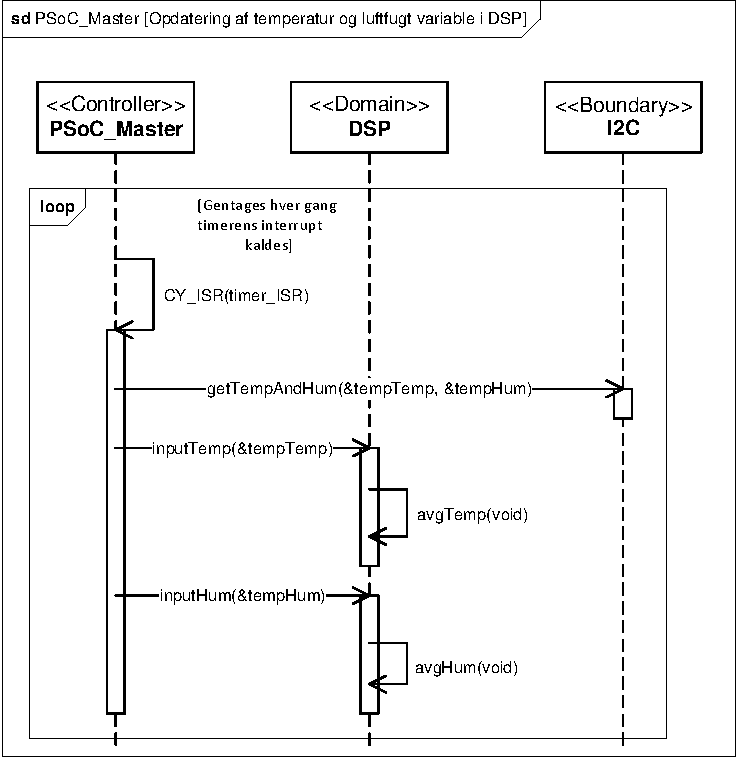
\includegraphics[scale=1]{../fig/sd_PSoC_master_update_sensor_values}
\caption{Sekvensdiagram over opdatering af sensorer.}
\label{fig:sd_PSoC_master_sensor}
\end{figure}

\begin{figure}[h]
\centering
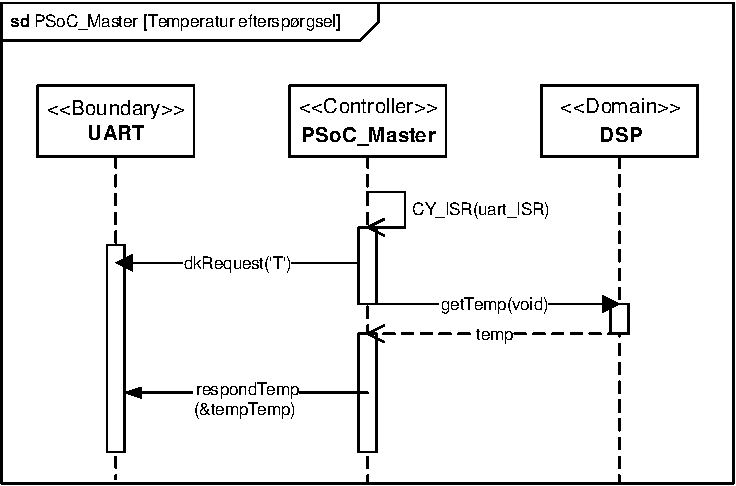
\includegraphics[scale=1]{../fig/sd_PSoC_master_tempreq}
\caption{Sekvensdiagram over forespørgsel af temperatur.}
\label{fig:sd_PSoC_master_tempreq}
\end{figure}

\begin{figure}[h]
\centering
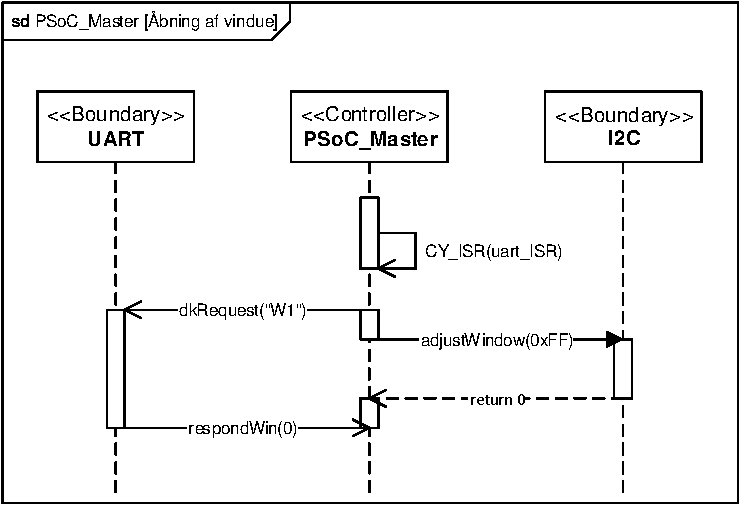
\includegraphics[scale=1]{../fig/sd_PSoC_master_open_window}
\caption{Sekvensdiagram over åbning af vindue.}
\label{fig:sd_PSoC_master_window}
\end{figure}



\clearpage